\documentclass[12pt]{article}
\usepackage[margin=2cm]{geometry}
\usepackage[utf8]{inputenc}

\title{Mutual Information between Categorical and Gaussian data}
\author{David Atienza}
\date{\today}

\usepackage{amsmath}
\usepackage{tikz}
\usetikzlibrary{positioning}
\usetikzlibrary{arrows.meta}

\usepackage{subfig}

\newcommand{\zd}{\mathbf{Z}_D}
\newcommand{\zc}{\mathbf{Z}_C}
\newcommand{\z}{\mathbf{Z}_D, \mathbf{Z}_C}


\begin{document}

\maketitle


\section{Introduction}

This documents shows how to calculate the (conditional) mutual information between categorical and Gaussian data. The mutual information is always calculated between two variables $X$ and $Y$, and can be conditioned on a set of variables $\mathbf{Z}$. Any of this variables can be discrete (categorical) or continuous (Gaussian). When needed, the subscript $D$ and $C$ are used to specify that the variable is discrete or continuous, e.g. $X_{D}$ is a discrete $X$ variable, $\mathbf{Z}_C$ is a set of conditioning continuous variables. The instantations for a given variable is denoted using lowercase, e.g. $x_d$, $y_c$, etc. The number of categories of the variables $X$ and $Y$ are denoted $\text{llx}$ and $\text{lly}$, respectively. The total number of categories for all the $\zd$ variables is denoted $\text{llz} = \prod_i \text{llz}_{i}$.

\section{Mutual Information}

\subsection{Mutual Information between Two Discrete Variables}

First we will calculate the mutual information between two discrete variables:

\begin{equation}
\begin{aligned}
I(X_D; Y_D \mid \z) & = H(X_D, \z) + H(Y_D, \z) - H(X_D, Y_D, \z) - H(\z)\\
& = H(\zc \mid X_D, \zd) + H(X_D, \zd) + H(\zc\mid Y_D, \zd) + H(Y_D, \zd)\\
&\phantom{ = }{}- H(\zc \mid X_D, Y_D, \zd) - H(X_D, Y_D, \zd) - H(\zc \mid \zd) - H(\zd)
\end{aligned}
\end{equation}

Note that:

\begin{equation}
I(X_D; Y_D \mid \zd) = H(X_D, \zd) + H(Y_D, \zd) - H(X_D, Y_D, \zd) - H(\zd)
\end{equation}

Thus:

\begin{equation}
\begin{aligned}
I(X_D; Y_D \mid \z) & = I(X_D; Y_D \mid \zd)\\
&\phantom{=}{} + H(\zc \mid X_D, \zd) + H(\zc\mid Y_D, \zd) - H(\zc \mid X_D, Y_D, \zd) - H(\zc \mid \zd)
\end{aligned}
\end{equation}

where $H(\zc \mid X_D, \zd)$ is the entropy of the Gaussian variables conditioned on $X_D, \zd$. This can be easily calculated:

\begin{equation}
\begin{aligned}
H(\zc \mid X_D, \zd) & = - \sum\limits_{x_d \in X_D, \mathbf{z}_d \in \zd} \int f(\zc, x_d, \mathbf{z}_d)\log\left(\frac{f(\zc, x_d, \mathbf{z}_d)}{f(x_d, \mathbf{z}_d)}\right)d\zc\\
& = - \sum\limits_{x_d \in X_D, \mathbf{z}_d \in \zd} p(x_d, \mathbf{z}_d) \int f(\zc \mid x_d, \mathbf{z}_d)\log\left(f(\zc \mid x_d, \mathbf{z}_d)\right)d\zc\\
& = \sum\limits_{x_d \in X_D, \mathbf{z}_d \in \zd} p(x_d, \mathbf{z}_d) H(\zc \mid x_d, \mathbf{z}_d)
\end{aligned}
\label{eq:conditional_entropy}
\end{equation}

The last integral in (\ref{eq:conditional_entropy}) is the entropy of the Gaussian distribution trained with the $x_d, \mathbf{z}_d$ configuration.

For a Gaussian distribution, this integral can be solved with a closed-form formula:

\begin{equation}
H(\zc \mid x_d, \mathbf{z}_d) = \frac{k}{2} + \frac{k}{2}\log(2\pi) + \frac{1}{2}\log(\lvert\boldsymbol{\Sigma}_{x_d, \mathbf{z}_d}\rvert)
\end{equation}
where $k = \lvert\zc\rvert$ is the dimensionality of the Gaussian distribution and $\boldsymbol{\Sigma}_{x_d, \mathbf{z}_d}$ is the covariance of the data with the discrete configuration $x_d, \mathbf{z}_d$.

The remaining terms $H(\zc \mid Y_D, \zd)$, $H(\zc \mid X_D, Y_D, \zd)$ and $H(\zc \mid \zd)$ can be calculated similarly.

\subsection{Mutual Information between a Discrete and Continuous Variable}

\begin{equation}
\begin{aligned}
I(X_D; Y_C \mid \z) & = H(X_D, \z) + H(Y_C, \z) - H(X_D, Y_C, \z) - H(\z)\\
& = H(\zc \mid X_D, \zd) + H(X_D, \zd) + H(Y_C, \zc\mid \zd) + H(\zd)\\
&\phantom{ = }{}- H(Y_C, \zc \mid X_D, \zd) - H(X_D, \zd) - H(\zc \mid \zd) - H(\zd)\\
& = H(\zc \mid X_D, \zd) + H(Y_C, \zc\mid \zd) - H(Y_C, \zc \mid X_D, \zd) - H(\zc \mid \zd)
\end{aligned}
\end{equation}
where the entropy terms can be calculated as in (\ref{eq:conditional_entropy}), but in this case the variable $Y$ is added in some of the estimated multivariate Gaussian distributions.

\subsection{Mutual Information between Two Continuous Variable}

For an unconditional mutual information, the mutual information can be calculated with the correlation coefficient:

\begin{equation}
I(X_C; Y_C) = -\frac{1}{2}\log\left(1-\rho^2\right)
\end{equation}
where $\rho$ is the linear correlation coefficient between $X$ and $Y$.

For the general case:

\begin{equation}
\begin{aligned}
I(X_C; Y_C \mid \z) & = H(X_C, \z) + H(Y_C, \z) - H(X_C, Y_C, \z) - H(\z)\\
& = H(X_C, \zc \mid \zd) + H(\zd) + H(Y_C, \zc\mid \zd) + H(\zd)\\
&\phantom{ = }{}- H(X_C, Y_C, \zc \mid \zd) - H(\zd) - H(\zc \mid \zd) - H(\zd)\\
& = H(X_C, \zc \mid \zd) + H(Y_C, \zc\mid \zd) - H(X_C, Y_C, \zc \mid \zd) - H(\zc \mid \zd)
\end{aligned}
\end{equation}
where the entropy terms can be calculated as in (\ref{eq:conditional_entropy}), but in this case the variables $X$ and $Y$ are added in some of the estimated multivariate Gaussian distributions.


\section{Empirical Degrees of Freedom}

This section shows the empirical degrees of freedom by running a simulation over 1000 datasets of 100000 instances that are compatible with the null hypothesis (conditional independence). The empirical degrees of freedom have been rounded to the nearest integer number.

\subsection{Empirical Degrees of Freedom between Two Discrete Variables}

\begin{table}[h]
\begin{center}
\begin{tabular}{ccccccccccccccccccc}
\multicolumn{4}{c}{1 cont. parents} & &\multicolumn{4}{c}{2 cont. parents} & &\multicolumn{4}{c}{3 cont. parents} & & \multicolumn{4}{c}{4 cont. parents}\\
llx & lly & llz & df & & llx & lly  & llz & df & & llx & lly & llz & df & & llx & lly  & llz & df\\
2 & 4 & 3 & 18 & & 2 & 4 & 3 & 36 & & 2 & 4 & 3 & 63 & & 2 & 4 & 3 & 99\\
2 & 3 & 4 & 16 & & 2 & 3 & 4 & 32 & & 2 & 3 & 4 & 56 & & 2 & 3 & 4 & 88\\
3 & 4 & 2 & 24 & & 3 & 4 & 2 & 48 & & 3 & 4 & 2 & 84 & & 3 & 4 & 2 & 132
\end{tabular}
\end{center}
\end{table}

Inducted formula:

\begin{equation}
\text{df} = (\text{llx} - 1)\cdot(\text{lly} - 1)\cdot\text{llz}\cdot\left[1 + \frac{\lvert\zc\rvert\cdot(\lvert\zc\rvert + 1)}{2}\right]
\end{equation}


\subsection{Empirical Degrees of Freedom between a Discrete and Continuous Variable}

\begin{table}[h]
\begin{center}
\begin{tabular}{ccccccccccccccccccc}
\multicolumn{4}{c}{1 cont. parents} & &\multicolumn{4}{c}{2 cont. parents} & &\multicolumn{4}{c}{3 cont. parents} & & \multicolumn{4}{c}{4 cont. parents}\\
llx & conty & llz & df & & llx & conty  & llz & df & & llx & conty & llz & df & & llx & conty  & llz & df\\
2 & & 3 & 6 & & 2 & & 3 & 9 & & 2 & & 3 & 12 & & 2 & & 3 & 15\\
2 & & 4 & 8 & & 2 & & 4 & 12 & & 2 & & 4 & 16 & & 2 & & 4 & 20\\
3 & & 2 & 8 & & 3 & & 2 & 12 & & 3 & & 2 & 16 & & 3 & & 2 & 20\\
3 & & 4 & 16 & & 3 & & 4 & 24 & & 3 & & 4 & 32 & & 3 & & 4 & 40\\
4 & & 2 & 12 & & 4 & & 2 & 18 & & 4 & & 2 & 24 & & 4 & & 2 & 30\\
4 & & 3 & 18 & & 4 & & 3 & 27 & & 4 & & 3 & 36 & & 4 & & 3 & 45
\end{tabular}
\end{center}
\end{table}

Inducted formula:

\begin{equation}
\text{df} = (\text{llx} - 1)\cdot\text{llz}\cdot\left[1 + \lvert\zc\rvert\right]
\end{equation}

\subsection{Empirical Degrees of Freedom between Two Continuous Variables}

\begin{table}[h]
\begin{center}
\begin{tabular}{ccccccccccccccccccc}
\multicolumn{4}{c}{1 cont. parents} & &\multicolumn{4}{c}{2 cont. parents} & &\multicolumn{4}{c}{3 cont. parents} & & \multicolumn{4}{c}{4 cont. parents}\\
contx & conty & llz & df & & contx & conty  & llz & df & & contx & conty & llz & df & & contx & conty  & llz & df\\
 & & 2 & 2 & & & & 2 & 2 & & & & 2 & 2 & & & & 2 & 2\\
 & & 3 & 3 & & & & 3 & 3 & & & & 3 & 3 & & & & 3 & 3\\
 & & 4 & 4 & & & & 4 & 4 & & & & 4 & 4 & & & & 4 & 4
\end{tabular}
\end{center}
\end{table}

Inducted formula:

\begin{equation}
\text{df} = \text{llz}
\end{equation}

\section{Asymptotic Degrees of Freedom}

\subsection{Asymptotic Degrees of Freedom between Two Discrete Variables}

There is a direct relationship between mutual information and a likelihood ratio test ($G$-test):

\begin{equation}
G = 2\cdot N\cdot I(X_D; Y_D \mid \z)
\end{equation}

The $G$ statistic is distributed as a $\chi^2$ if the null hypothesis is true. The degrees of freedom of the $\chi^2$ distribution is the difference in the number of free parameters between a model where there is conditional dependence between $X_D$ and $Y_D$ (Figure~\ref{fig:h1_discrete}), and a model where there is no conditional dependence between $X_D$ and $Y_D$  (Figure~\ref{fig:h0_discrete}).

\begin{figure}
\begin{center}
\subfloat[$H_{0}$ model] {
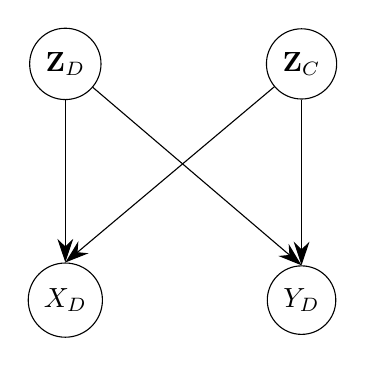
\begin{tikzpicture}
    \node[shape=circle,draw=black] (Z_D) at (0,3) {$\zd$};
    \node[shape=circle,draw=black] (Z_C) at (3,3) {$\zc$};
    \node[shape=circle,draw=black] (X_D) at (0,0) {$X_D$};
    \node[shape=circle,draw=black] (Y_D) at (3,0) {$Y_D$};
    
    
    \draw [-{Stealth[length=3mm, width=2mm]}] (Z_D) edge (X_D.north);
    \path [-{Stealth[length=3mm, width=2mm]}] (Z_D) edge (Y_D.north);
    
    \path [-{Stealth[length=3mm, width=2mm]}] (Z_C) edge (X_D.north);
    \path [-{Stealth[length=3mm, width=2mm]}] (Z_C) edge (Y_D.north);
\end{tikzpicture}
\label{fig:h0_discrete}
}
\hspace{3cm}
\subfloat[$H_{1}$ model] {
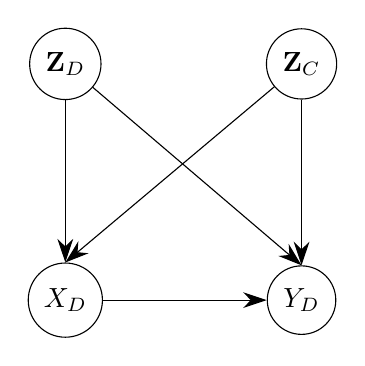
\begin{tikzpicture}
    \node[shape=circle,draw=black] (Z_D) at (0,3) {$\zd$};
    \node[shape=circle,draw=black] (Z_C) at (3,3) {$\zc$};
    \node[shape=circle,draw=black] (X_D) at (0,0) {$X_D$};
    \node[shape=circle,draw=black] (Y_D) at (3,0) {$Y_D$};
    
    
    \draw [-{Stealth[length=3mm, width=2mm]}] (Z_D) edge (X_D.north);
    \path [-{Stealth[length=3mm, width=2mm]}] (Z_D) edge (Y_D.north);
    
    \path [-{Stealth[length=3mm, width=2mm]}] (Z_C) edge (X_D.north);
    \path [-{Stealth[length=3mm, width=2mm]}] (Z_C) edge (Y_D.north);
    \path [-{Stealth[length=3mm, width=2mm]}] (X_D.east) edge (Y_D.west);
\end{tikzpicture}
\label{fig:h1_discrete}
}
\end{center}
\caption{Null hypothesis (left) and alternative (right) models for two discrete variables.}
\end{figure}

The only node that contains a different number of parameters is the conditional distribution of $Y_D$. So we must analyze that distribution to find the degrees of freedom of the $\chi^2$ distribution.

For the $H_0$ model, the distribution $f(Y_D \mid \z)$ can be defined using the Bayes rule (as in a conditional linear Gaussian networks the discrete nodes do not have continuous parents):

\begin{equation}
f(Y_D \mid \z) = \frac{f(\zc \mid Y_D, \zd) f(Y_D \mid \zd)}{f(\zc \mid \zd)}
\end{equation}

Note that only $\text{lly} - 1$ models are needed to be fitted because the probabilities $f(Y_D \mid \z)$ must sum to 1, so the probability for the last category can be defined as:

\begin{equation}
f(Y_D = \text{lly}\mid \z) = 1 - \sum\limits_{i = 1}^{\text{lly} - 1}\frac{f(\zc \mid Y_D = i, \zd) f(Y_D = i \mid \zd)}{f(\zc \mid \zd)}
\end{equation}


$f(\zc \mid Y_D, \zd)$ has  a number of free parameters equal to:

\begin{equation}
(\text{lly} - 1)\cdot\text{llz}\cdot\frac{\lvert\zc\rvert\cdot(\lvert\zc\rvert + 3)}{2}
\end{equation}

Note that $\frac{\lvert\zc\rvert\cdot(\lvert\zc\rvert + 3)}{2}$ is the number of free parameters of a multivariate Gaussian distribution of $\lvert\zc\rvert$ dimensions.

$f(Y_D \mid \zd)$ has a number of free parameters equal to:

\begin{equation}
(\text{lly} - 1)\cdot \text{llz}
\end{equation}

$f(\zc \mid \zd)$ does not contain free parameters because it can be represented using the previous functions:

\begin{equation}
f(\zc \mid \zd) = \sum\limits_{y_d \in Y_D} f(\zc \mid Y_D = y_d, \zd) f(Y_D = y_d \mid \zd)
\end{equation}

For the $H_1$ model, the distribution $f(Y_D \mid X_D, \z)$ can be defined using the Bayes rule (as in a conditional linear Gaussian networks the discrete nodes do not have continuous parents):

\begin{equation}
f(Y_D \mid X_D, \z) = \frac{f(\zc \mid X_D, Y_D, \zd) f(Y_D \mid X_D, \zd)}{f(\zc \mid X_D, \zd)}
\end{equation}

Note that only $\text{lly} - 1$ models are needed to be fitted because the probabilities $f(Y_D \mid X_D, \z)$ must sum to 1, so the probability for the last category can be defined as:

\begin{equation}
f(Y_D = \text{lly}\mid X_D, \z) = 1 - \sum\limits_{i = 1}^{\text{lly} - 1}\frac{f(\zc \mid X_D, Y_D = i, \zd) f(Y_D = i \mid X_D, \zd)}{f(\zc \mid X_D, \zd)}
\end{equation}


$f(\zc \mid X_D, Y_D, \zd)$ has  a number of free parameters equal to:

\begin{equation}
(\text{lly} - 1)\cdot\text{llx}\cdot\text{llz}\cdot\frac{\lvert\zc\rvert\cdot(\lvert\zc\rvert + 3)}{2}
\end{equation}


$f(Y_D \mid X_D, \zd)$ has a number of free parameters equal to:

\begin{equation}
(\text{lly} - 1)\cdot\text{llx}\cdot\text{llz}
\end{equation}

$f(\zc \mid X_D, \zd)$ does not contain free parameters because it can be represented using the previous functions:

\begin{equation}
f(\zc \mid X_D, \zd) = \sum\limits_{y_d \in Y_D} f(\zc \mid X_D, Y_D = y_d, \zd) f(Y_D = y_d \mid X_D, \zd)
\end{equation}

The difference in parameters (and the degrees of freedom of the $\chi^2$) is equal to:

\begin{equation}
\begin{aligned}
\text{df} & = \text{lly} - 1)\cdot(\text{llx} - 1)\cdot\text{llz}\cdot\frac{\lvert\zc\rvert\cdot(\lvert\zc\rvert + 3)}{2} + (\text{lly} - 1)\cdot(\text{llx}-1)\cdot\text{llz}\\
& = \boxed{(\text{lly} - 1)\cdot(\text{llx}-1)\cdot\text{llz}\left[1 + \frac{\lvert\zc\rvert\cdot(\lvert\zc\rvert + 3)}{2}\right]}
\end{aligned}
\end{equation}

\subsection{Asymptotic Degrees of Freedom between a Discrete and Continuous Variable}

The $H_{0}$ model is shown in Figure~\ref{fig:h0_mixed} and the $H_{1}$ model is shown in Figure~\ref{fig:h1_mixed}.

\begin{figure}
\begin{center}
\subfloat[$H_{0}$ model] {
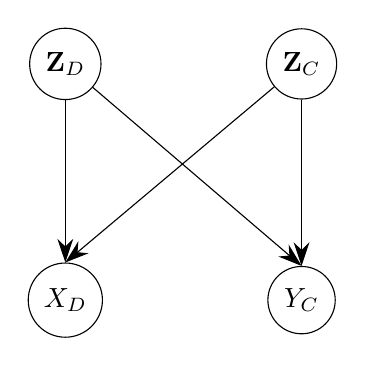
\begin{tikzpicture}
    \node[shape=circle,draw=black] (Z_D) at (0,3) {$\zd$};
    \node[shape=circle,draw=black] (Z_C) at (3,3) {$\zc$};
    \node[shape=circle,draw=black] (X_D) at (0,0) {$X_D$};
    \node[shape=circle,draw=black] (Y_D) at (3,0) {$Y_C$};
    
    
    \draw [-{Stealth[length=3mm, width=2mm]}] (Z_D) edge (X_D.north);
    \path [-{Stealth[length=3mm, width=2mm]}] (Z_D) edge (Y_D.north);
    
    \path [-{Stealth[length=3mm, width=2mm]}] (Z_C) edge (X_D.north);
    \path [-{Stealth[length=3mm, width=2mm]}] (Z_C) edge (Y_D.north);
\end{tikzpicture}
\label{fig:h0_mixed}
}
\hspace{3cm}
\subfloat[$H_{1}$ model] {
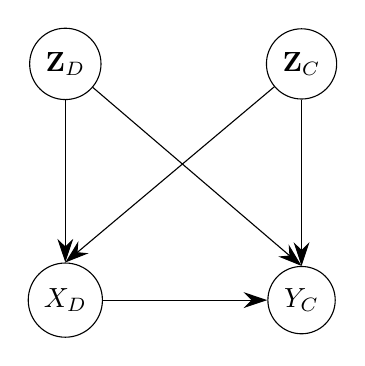
\begin{tikzpicture}
    \node[shape=circle,draw=black] (Z_D) at (0,3) {$\zd$};
    \node[shape=circle,draw=black] (Z_C) at (3,3) {$\zc$};
    \node[shape=circle,draw=black] (X_D) at (0,0) {$X_D$};
    \node[shape=circle,draw=black] (Y_D) at (3,0) {$Y_C$};
    
    
    \draw [-{Stealth[length=3mm, width=2mm]}] (Z_D) edge (X_D.north);
    \path [-{Stealth[length=3mm, width=2mm]}] (Z_D) edge (Y_D.north);
    
    \path [-{Stealth[length=3mm, width=2mm]}] (Z_C) edge (X_D.north);
    \path [-{Stealth[length=3mm, width=2mm]}] (Z_C) edge (Y_D.north);
    \path [-{Stealth[length=3mm, width=2mm]}] (X_D.east) edge (Y_D.west);
\end{tikzpicture}
\label{fig:h1_mixed}
}
\end{center}
\caption{Null hypothesis (left) and alternative (right) models for a continuous and discrete variable.}
\end{figure}

The distribution $f(Y_C \mid \z)$ has a number of free parameters equal to:

\begin{equation}
\text{llz}\cdot\left(\lvert\zc\rvert + 2\right)
\end{equation}


The distribution $f(Y_C \mid X_D, \z)$ has a number of free parameters equal to:

\begin{equation}
\text{llx}\cdot\text{llz}\cdot\left(\lvert\zc\rvert + 2\right)
\end{equation}

The difference in parameters (and the degrees of freedom of the $\chi^2$) is equal to:

\begin{equation}
\boxed{\text{df} = (\text{llx}-1)\cdot\text{llz}\cdot\left(\lvert\zc\rvert + 2\right)}
\end{equation}

The same result can be derived using a different $H_0$ model (Figure~\ref{fig:h0_mixed2}) and $H_1$ model (Figure~\ref{fig:h1_mixed2}). In this case, the difference in the number of parameters happens to be in the conditional distribution of $X_D$.

\begin{figure}
\begin{center}
\subfloat[$H_{0}$ model] {
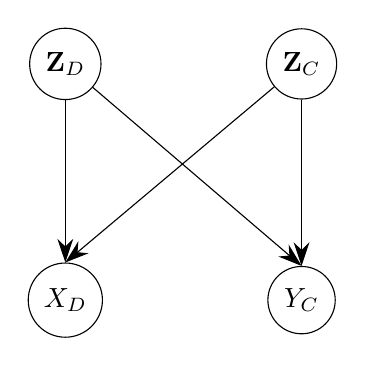
\begin{tikzpicture}
    \node[shape=circle,draw=black] (Z_D) at (0,3) {$\zd$};
    \node[shape=circle,draw=black] (Z_C) at (3,3) {$\zc$};
    \node[shape=circle,draw=black] (X_D) at (0,0) {$X_D$};
    \node[shape=circle,draw=black] (Y_D) at (3,0) {$Y_C$};
    
    
    \draw [-{Stealth[length=3mm, width=2mm]}] (Z_D) edge (X_D.north);
    \path [-{Stealth[length=3mm, width=2mm]}] (Z_D) edge (Y_D.north);
    
    \path [-{Stealth[length=3mm, width=2mm]}] (Z_C) edge (X_D.north);
    \path [-{Stealth[length=3mm, width=2mm]}] (Z_C) edge (Y_D.north);
\end{tikzpicture}
\label{fig:h0_mixed2}
}
\hspace{3cm}
\subfloat[$H_{1}$ model] {
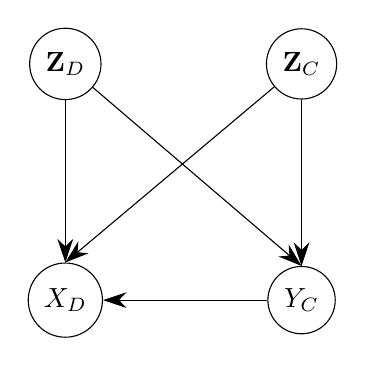
\begin{tikzpicture}
    \node[shape=circle,draw=black] (Z_D) at (0,3) {$\zd$};
    \node[shape=circle,draw=black] (Z_C) at (3,3) {$\zc$};
    \node[shape=circle,draw=black] (X_D) at (0,0) {$X_D$};
    \node[shape=circle,draw=black] (Y_D) at (3,0) {$Y_C$};
    
    
    \draw [-{Stealth[length=3mm, width=2mm]}] (Z_D) edge (X_D.north);
    \path [-{Stealth[length=3mm, width=2mm]}] (Z_D) edge (Y_D.north);
    
    \path [-{Stealth[length=3mm, width=2mm]}] (Z_C) edge (X_D.north);
    \path [-{Stealth[length=3mm, width=2mm]}] (Z_C) edge (Y_D.north);
    \path [-{Stealth[length=3mm, width=2mm]}] (Y_D.west) edge (X_D.east);
\end{tikzpicture}
\label{fig:h1_mixed2}
}
\end{center}
\caption{Variation of the null hypothesis (left) and alternative (right) models for a continuous and discrete variable.}
\end{figure}

The $f(X_D\mid \z)$ can be defined using the Bayes rule:

\begin{equation}
f(X_D\mid\z) = \frac{f(\zc\mid X_D, \zd)f(X_D\mid \zd)}{f(\zc\mid\zd)}
\end{equation}

Note that only $\text{llx} - 1$ models are needed to be fitted because the probabilities $f(X_D \mid \z)$ must sum to 1, so the probability for the last category can be defined as:

\begin{equation}
f(X_D = \text{llx}\mid \z) = 1 - \sum\limits_{i = 1}^{\text{llx} - 1}\frac{f(\zc \mid X_D = i, \zd) f(X_D = i \mid \zd)}{f(\zc \mid\zd)}
\end{equation}

The distribution $f(\zc\mid X_D, \zd)$ has a number of free parameters equal to:

\begin{equation}
(\text{llx} - 1)\cdot\text{llz}\cdot\frac{\lvert\zc\rvert\cdot(\lvert\zc\rvert + 3)}{2}
\end{equation}

The distribution $f(X_D\mid \zd)$ has a number of free parameters equal to:

\begin{equation}
(\text{llx} - 1)\cdot\text{llz}
\end{equation}

$f(\zc \mid\zd)$ does not contain free parameters because it can be represented using the previous functions:

\begin{equation}
f(\zc \mid \zd) = \sum\limits_{x_d \in X_D} f(\zc \mid X_D = x_d, \zd) f(X_D = x_d \mid \zd)
\end{equation}


The $f(X_D\mid \z)$ can be defined using the Bayes rule:

\begin{equation}
f(X_D\mid Y_C, \z) = \frac{f(Y_C, \zc\mid X_D, \zd)f(X_D\mid \zd)}{f(Y_C, \zc\mid\zd)}
\end{equation}


Note that only $\text{llx} - 1$ models are needed to be fitted because the probabilities $f(X_D \mid Y_C, \z)$ must sum to 1, so the probability for the last category can be defined as:

\begin{equation}
f(X_D = \text{llx}\mid Y_C, \z) = 1 - \sum\limits_{i = 1}^{\text{llx} - 1}\frac{f(Y_C, \zc \mid X_D = i, \zd) f(X_D = i \mid \zd)}{f(Y_C,\zc \mid\zd)}
\end{equation}

The distribution $f(Y_C, \zc\mid X_D, \zd)$ has a number of free parameters equal to:

\begin{equation}
(\text{llx} - 1)\cdot\text{llz}\cdot\frac{\left(\lvert\zc\rvert + 1\right)\cdot\left(\lvert\zc\rvert + 4\right)}{2}
\end{equation}

The distribution $f(X_D\mid \zd)$ has a number of free parameters equal to:

\begin{equation}
(\text{llx} - 1)\cdot\text{llz}
\end{equation}

$f(\zc \mid\zd)$ does not contain free parameters because it can be represented using the previous functions:

\begin{equation}
f(Y_C, \zc \mid \zd) = \sum\limits_{x_d \in X_D} f(Y_C, \zc \mid X_D = x_d, \zd) f(X_D = x_d \mid \zd)
\end{equation}

The difference in parameters (and the degrees of freedom of the $\chi^2$) is equal to:

\begin{equation}
\begin{aligned}
\text{df} & = (\text{llx}-1)\cdot\text{llz}\cdot\left(\frac{\lvert\zc\rvert^{2} + 5\lvert\zc\rvert + 4 - \lvert\zc\rvert^{2} - 3\lvert\zc\rvert}{2}\right)\\
& = (\text{llx}-1)\cdot\text{llz}\cdot\left(\frac{2\lvert\zc\rvert + 4}{2}\right)\\
& = \boxed{(\text{llx}-1)\cdot\text{llz}\cdot\left(\lvert\zc\rvert + 2\right)}
\end{aligned}
\end{equation}

\subsection{Asymptotic Degrees of Freedom between Two Continuous Variables}

The $H_{0}$ model is shown in Figure~\ref{fig:h0_cont} and the $H_{1}$ model is shown in Figure~\ref{fig:h1_cont}.



\begin{figure}
\begin{center}
\subfloat[$H_{0}$ model] {
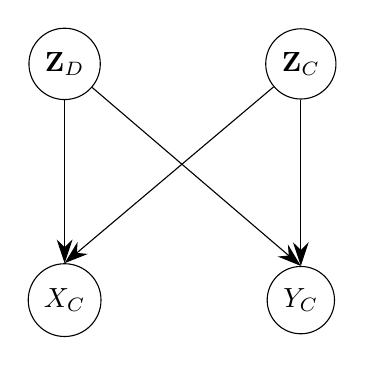
\begin{tikzpicture}
    \node[shape=circle,draw=black] (Z_D) at (0,3) {$\zd$};
    \node[shape=circle,draw=black] (Z_C) at (3,3) {$\zc$};
    \node[shape=circle,draw=black] (X_D) at (0,0) {$X_C$};
    \node[shape=circle,draw=black] (Y_D) at (3,0) {$Y_C$};
    
    
    \draw [-{Stealth[length=3mm, width=2mm]}] (Z_D) edge (X_D.north);
    \path [-{Stealth[length=3mm, width=2mm]}] (Z_D) edge (Y_D.north);
    
    \path [-{Stealth[length=3mm, width=2mm]}] (Z_C) edge (X_D.north);
    \path [-{Stealth[length=3mm, width=2mm]}] (Z_C) edge (Y_D.north);
\end{tikzpicture}
\label{fig:h0_cont}
}
\hspace{3cm}
\subfloat[$H_{1}$ model] {
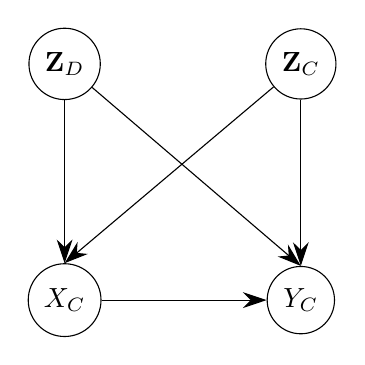
\begin{tikzpicture}
    \node[shape=circle,draw=black] (Z_D) at (0,3) {$\zd$};
    \node[shape=circle,draw=black] (Z_C) at (3,3) {$\zc$};
    \node[shape=circle,draw=black] (X_D) at (0,0) {$X_C$};
    \node[shape=circle,draw=black] (Y_D) at (3,0) {$Y_C$};
    
    
    \draw [-{Stealth[length=3mm, width=2mm]}] (Z_D) edge (X_D.north);
    \path [-{Stealth[length=3mm, width=2mm]}] (Z_D) edge (Y_D.north);
    
    \path [-{Stealth[length=3mm, width=2mm]}] (Z_C) edge (X_D.north);
    \path [-{Stealth[length=3mm, width=2mm]}] (Z_C) edge (Y_D.north);
    \path [-{Stealth[length=3mm, width=2mm]}] (X_D.east) edge (Y_D.west);
\end{tikzpicture}
\label{fig:h1_cont}
}
\end{center}
\caption{Null hypothesis (left) and alternative (right) models for two continuous variables.}
\end{figure}


For the $H_0$ model, the distribution $f(Y_C\mid \z)$ has a number of free parameters equal to:

\begin{equation}
\text{llz}\cdot\left(\lvert\zc\rvert + 2\right)
\end{equation}

For the $H_1$ model, the distribution $f(Y_C\mid X_C, \z)$ has a number of free parameters equal to:

\begin{equation}
\text{llz}\cdot\left(\lvert\zc\rvert + 3\right)
\end{equation}

The difference in parameters (and the degrees of freedom of the $\chi^2$) is equal to:

\begin{equation}
\boxed{\text{llz}}
\end{equation}



\end{document}